%%%%%%%%%%%%%%%%%%%%%%%%%%%%%%%%%%%%%%%%%%%%%%%%%%%%%%%%%%%%%%%%%%%%%%
%%                     Inhibition
%%%%%%%%%%%%%%%%%%%%%%%%%%%%%%%%%%%%%%%%%%%%%%%%%%%%%%%%%%%%%%%%%%%%%%

\subsection{Glyph: \glyph{Inhibition}}\label{sec:inhibition}
\color{blue}

An inhibition \textbf{negatively}  the the strength, or the probability, of the target relationship. 

\begin{glyphDescription}
 \glyphSboTerm SBO:0000169 ! inhibition.
 \glyphOrigin Any \glyph{interactor} (\sect{interactors}) or any \glyph{logical operator} (\sect{logic}).
 \glyphTarget Any \glyph{statement} (\sect{statements}) or \glyph{influence} (\sect{influences}).
 \glyphEndPoint The target extremity of a \glyph{inhibitiom} carries a bar perpendicular to the arc.
 \end{glyphDescription}

\begin{figure}[H]
  \centering
  \includegraphics[scale = 0.5]{images/inhibition}
  \caption{The \PD glyph for \glyph{inhibition}.}
  \label{fig:inhibition}
\end{figure}

